\medskip

On considère la fonction $f$ définie sur l'intervalle $] 0~;~+\infty[$ par 
\[f(x) = (2-\ln x) \times \ln x,\]

où $\ln$ désigne la fonction logarithme népérien.

On admet que la fonction $f$ est deux fois dérivable sur $]0~;~+\infty[$.

On note $C$ la courbe représentative de la fonction $f$ dans un repère orthogonal et $C'$ la courbe représentative de la fonction $f'$, fonction dérivée de la fonction $f$.

La \textbf{courbe} $\boldsymbol{C}'$ est donnée ci-dessous ainsi que son unique tangente horizontale (T).

\begin{center}
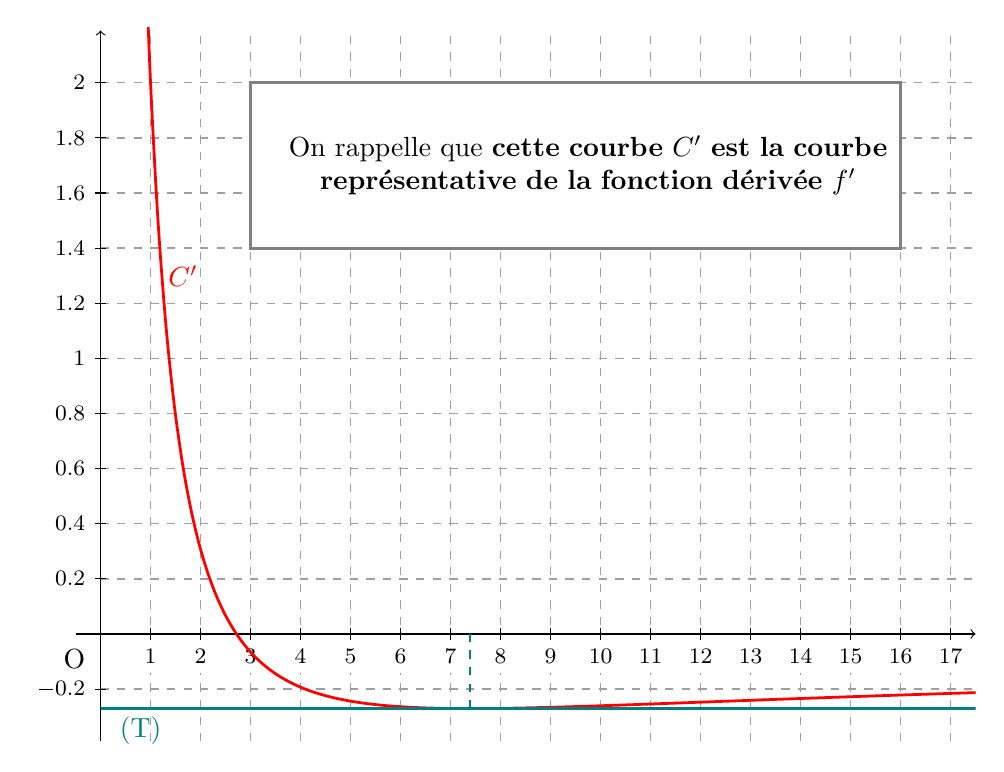
\begin{tikzpicture}[x=6.35mm,y=35mm]






	\draw [color = gray!75, line width = 0.5pt, xstep=1, ystep = 0.2,dashed] (0,-0.39) grid (17.5,2.19);
\draw[->] (-0.5,0) -- (17.5,0);
\foreach \x in {1,...,17}
\draw[shift={(\x,0)},color=black] (0pt,2pt) -- (0pt,-2pt) node[below, fill = white] {\footnotesize $\np{\x}$};
\draw[->] (0,-0.39) -- (0,2.19);
\foreach \y in {-0.2,0.2,0.4,0.6,0.8,1,1.2,1.4,1.6,1.8,2}
\draw[shift={(0,\y)},color=black] (2pt,0pt) -- (-2pt,0pt) node[left, fill = white] {\footnotesize $\np{\y}$};
\draw[color=black] (-2pt,-2pt) node[below left] {O};
\clip (0,2.2) rectangle (17.5,-0.4);
\draw[line width=1pt,color=red,smooth,samples=100,domain= 0.8:17.5 ] plot(\x,{2*(1 - ln(\x))/\x} );
\node[red] at(1.65,1.3){$C'$};
\draw[teal,line width=1pt] (-0.5,-0.2707)--(17.5,-0.2707) ;
\draw[teal,line width=1pt,dashed] (7.3891,-0.2707)--(7.3891,0) ;
\node[teal] at(0.8,-0.35)  {(T)};
\draw[fill=white,draw=gray,line width=1pt] (3,1.4)rectangle(16,2); \node[text width=8.2cm,align=center] at (9.75,1.7){On rappelle que \textbf{cette courbe $C'$ est la courbe représentative de la fonction dérivée $f'$}} ;
\end{tikzpicture}
\end{center}


\begin{enumerate}
	\item Par lecture graphique, avec la précision que permet le tracé ci-dessus, donner :

	\begin{enumerate}
		\item le coefficient directeur de la tangente à $C$ au point d'abscisse 1.

		\item 	le plus grand intervalle sur lequel la fonction $f$ est convexe.
	\end{enumerate}

	\item \begin{enumerate}
		\item Calculer la limite de la fonction $f$ en $+\infty$.

		\item Calculer $\lim\limits_{x \to 0} f(x)$. Interpréter graphiquement ce résultat.
	\end{enumerate}

	\item Montrer que la courbe $C$ coupe l'axe des abscisses en deux points exactement dont on précisera les coordonnées.

	\item \begin{enumerate}
		\item Montrer que pour tout réel $x$ appartenant à $]0~;~+\infty[, \quad f'(x) = \dfrac{2(1-\ln x)}{x}$.

		\item En déduire, en justifiant, le tableau de variations de la fonction $f$ sur $]0~;~+\infty[$.
	\end{enumerate}

	\item On note $f''$ la dérivée seconde de $f$ et on admet que pour tout réel $x$ appartenant à $]0~;~+\infty[$, $f''(x) = \dfrac{2(\ln x-2)}{x^{2}}$.

Déterminer par le calcul le plus grand intervalle sur lequel la fonction $f$ est convexe et préciser les coordonnées du point d'inflexion de la courbe $C$.
\end{enumerate}

\vspace{1cm}
